\documentclass[11pt, twoside, letterpaper]{article}
\usepackage[utf8]{inputenc}
\usepackage[margin=0.6in]{geometry}
\usepackage{geometry}                   % See geometry.pdf to learn the layout options. There are lots.
\usepackage[parfill]{parskip}       % Activate to begin paragraphs with an empty line rather than an indent
\usepackage{graphicx}       % Use pdf, png, jpg, or eps§ with pdflatex; use eps in DVI mode
\usepackage{amssymb}
\usepackage{amsmath}
\usepackage{placeins}

\title{EE105 MiniProject: AM Radio}
\author{Michael Lin and Jene Li}
\date{December 2013}

\begin{document}

\maketitle

\section{Topology}
\subsection{MOSFET vs BJT}

The first decision we made was to use MOSFETS rather than BJTs because while they had lower gain than BJTs (the $g_m$ of MOSFETS
is in the order of $10^{-3}$ compared to the BJT's $0.038$), the large gate impedance of MOS proved more attractive since we dont have to
worry much about impedance loading between stages. As for the specific MOS, we used the BS170 N-channel MOSFETs because they had high saturation
current capacity and, thus, a higher $g_m$ and gain.

\subsection{Amplifier topology trade offs}

\subsubsection{Cascode}
We used a total of 6 stages in our amplifier. Five common sources and one source follower.
Our first decision was to choose topologies to use for amplification. We first considered using a cascode stage because of 
its characteristically high gain and good frequency response (high bandwidth). However, due to the high gain of the cascode
it was very difficult to bias it correctly such that it would not rail. The possible cascode configuration is shown in Figure 2,
We need to choose R1 and R2 carefully such that the current being forced by both PMOS and NMOS current mirrors are the same.
Otherwise, the small difference in current will reflect as a voltage drop in one of the $r_o$s and the high gain of the cascode
will amplify and rail this difference.

\begin{figure}[htbp]
\begin{center}
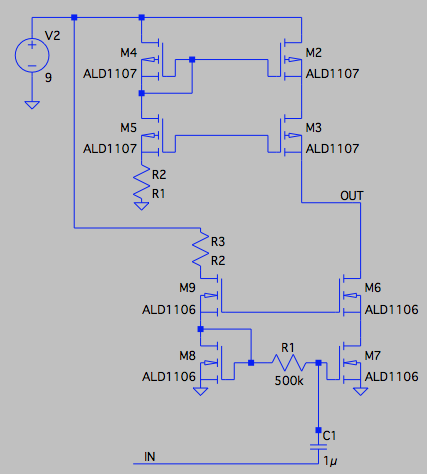
\includegraphics[width=4in,height=4in]{Cascode.png}
\caption{Cascode topology}
\end{center}
\end{figure}
\FloatBarrier

\subsubsection{Common Sources}
After some more consideration, we decided to use multiple stages of common source topologies as the one shown in Figure 3 because they would 
be much easier to bias than cascode stage. Our first decision was to choose a desired drain current and the gain and $V_{outBIAS}$
would depend on this current. We will go through this calculations in a later section, through educated guess and some trial and errors we 
chose a drain current of 6mA. Drain current is set by using a current mirror, as shown in Figure 3. Then we choose our drain 
resistance such that we get a well centered $V_{outBIAS}$. In our case, we chose $R_D=1000k\Omega$, so the voltage drop on the resistor would be 
6V and leave a $V_{outBIAS}\approx 4V$. The gain per common source stage turned out to be low due to this small $R_D$ and inconsistent across different 
BS170, probably due to their mismatch in $\frac{W}{L}$, in fact, it was a gain ranging from 5 to 10. However, since we did not have inter-stage loading 
gain loss due to the infinite gate impedance of the common sources, cascading multiple of this topologies increased our gain exponentially by a factor
of 5 to 10 every stage. So five stages were enough to reach a gain of over 12500. Besides the drain resistor, we also added a $100\Omega$ resistor 
at the source to stabilize the gate to source voltage.

\begin{figure}[htbp]
\begin{center}
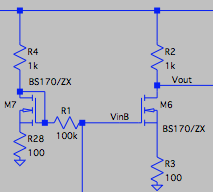
\includegraphics[width=3in,height=3in]{CurrentMirror.png}
\caption{Current Mirror Biasing a Common Source}
\end{center}
\end{figure}
\FloatBarrier

\subsection{Coupling between stages}

Between each of the common source stages we AC couple with a 10uF capacitor and individually bias the gate voltage of each stage with its own current 
mirror circuit as shown in Figure 1. Between the last common source M13 and the source follower M15 we use DC coupling as we will explain later on. 
And finally to drive the $8\Omega$ speaker we AC couple it so we dont drive it with a bias voltage otherwise it could sound distorted.

\subsection{Loading Stage}
The last stage of our amplifier is a Common Drain. We decided to use a common drain for multiple reasons. The first one and the main one
is that its output resistance is very small, approximately $\frac{1}{g_m}$. As we mentioned earlier our current of 6mA gives us a $g_m\approx10^{-3}s$
so the impedance looking into the source of the MOSFET is $\approx 1000\Omega$. Even though the gain of our source follower is approximately unity we
still have some gain loss since the load we are trying to drive is $8\Omega$ the voltage division will attenuate the signal by approximately 100=40dB 
however since the gain from our amplifier is high enough that our total circuit gain is just around 82dB which we will show later in the simulation 
and calculations. To drive our $8\Omega$ speaker with $1V_{pp}$ we use a $100\Omega$ resistor in parallel to draw some of the current and not burn 
the speaker with 1000/8=125mA. Another reason we use a source follower is that it has a good current gain, technically it has infinite current gain 
since there is no current going into the gate but the current throughput is enough to get it up to around 40mA to drive the speaker. We can see the 
implementation of the loading stage (source follower and speaker load) in Figure 4. To get a current as high as 40mA we had to bias the gate with a 
high enough voltage, so since the $V_{outBIAS}$ of the previous common source stage was already biased to around 4V, we decided to DC couple this 
last loading stage using the bias from the output of the last stage of common source as we can see in Figure 1.

\begin{figure}[htbp]
\begin{center}
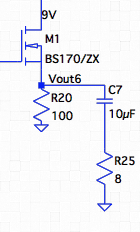
\includegraphics[width=2in,height=3in]{SourceFollower.png}
\caption{Source Follower: Loading Stage}
\end{center}
\end{figure}
\FloatBarrier

\subsection{Volume Control}
At last we implemented volume control using a potentiometer in the $R_D$ of the last common source stage as seen in Figure 5. We decided
to place the potentionmeter in the last stage because this is where the largest voltage swing happens and its easier to fine tune the 
voltage swing.

\begin{figure}[htbp]
\begin{center}
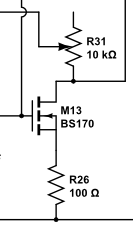
\includegraphics[width=2in,height=3in]{VolumeControl.png}
\caption{Volume Control on Last Common Source stage}
\end{center}
\end{figure}
\FloatBarrier

\subsection{Other small fixes to the amplifier}
Another problem we saw was that the power supply started getting very noisy probably due to feedback in the circuit or inappropriate capacitor
decoupling, this is an effect called "Squegging". Our solution to this was to add a 10uF capacitor in shunt with the power supply rails as 
seen in Figure 1 capacitor C9.
\newpage 

\section{Circuit Diagram}
\begin{figure}[htbp]
	\begin{center}
		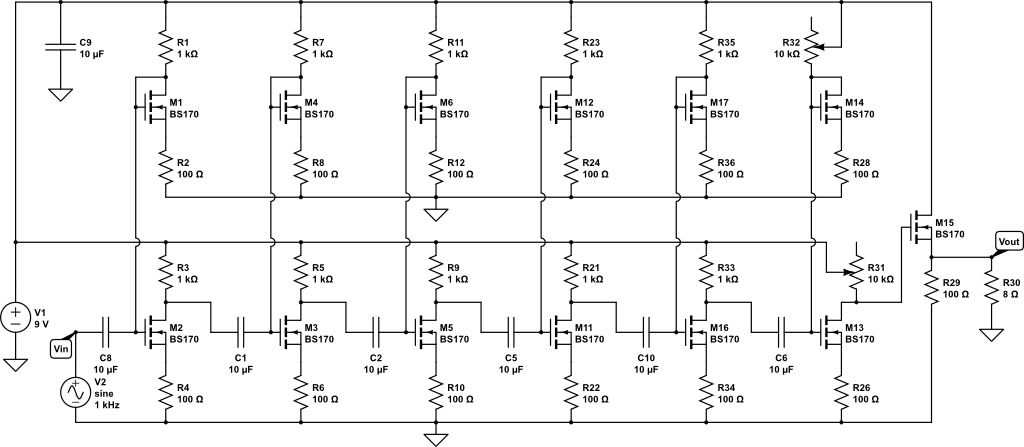
\includegraphics[scale=0.80,angle=-90]{circuitdiagram.png}
		\caption{Circuit Diagram}
	\end{center}
\end{figure}
\FloatBarrier
\newpage

\section{Hand Calculations and Measurements}
\subsection{Common Source Bias calculations}
Through educated guesses and some trials and errors we chose 6mA to be our drain current. From this we can calculate our theoretical bias voltage
$V_G$ for the current mirror shown in Figure 3. The current-voltage equation is given by

$I_d = \frac{1}{2} K_p (V_G - R_s I_d -V_{TO})^2 (1 + \lambda (V_G - R_s I_d))$
\begin{align*}
K_p &= 0.277\\
R_s &= 100\Omega\\
V_{TO} &= 1.8V\\
\lambda &= 0.003\\
I_d &= 6mA\\
6e-3 &= \frac{1}{2}0.277(V_G-0.6-1.8)^2(1+0.003(V_G-0.6))\\
V_G &= 2.6V
\end{align*}

\subsection*{Magnitude/Phase Bode Plot}

\begin{tabular}{|r|l|l|}
\hline
Frequency & Magnitude & Phase\\
\hline
$1$ kHz & 91.25 dBV & 180 \\
$2.8$ kHz & 90.89 dBV & 200 \\
$4.6$ kHz & 90.89 dBV & 200 \\
$6.4$ kHz& 93.07 dBV & 200 \\
$8.2$ kHz & 92.62 dBV & 200 \\
$10$  kHz& 93.07 dBV & 200 \\
\hline
\end{tabular}

\begin{figure}[htbp]
\begin{center}
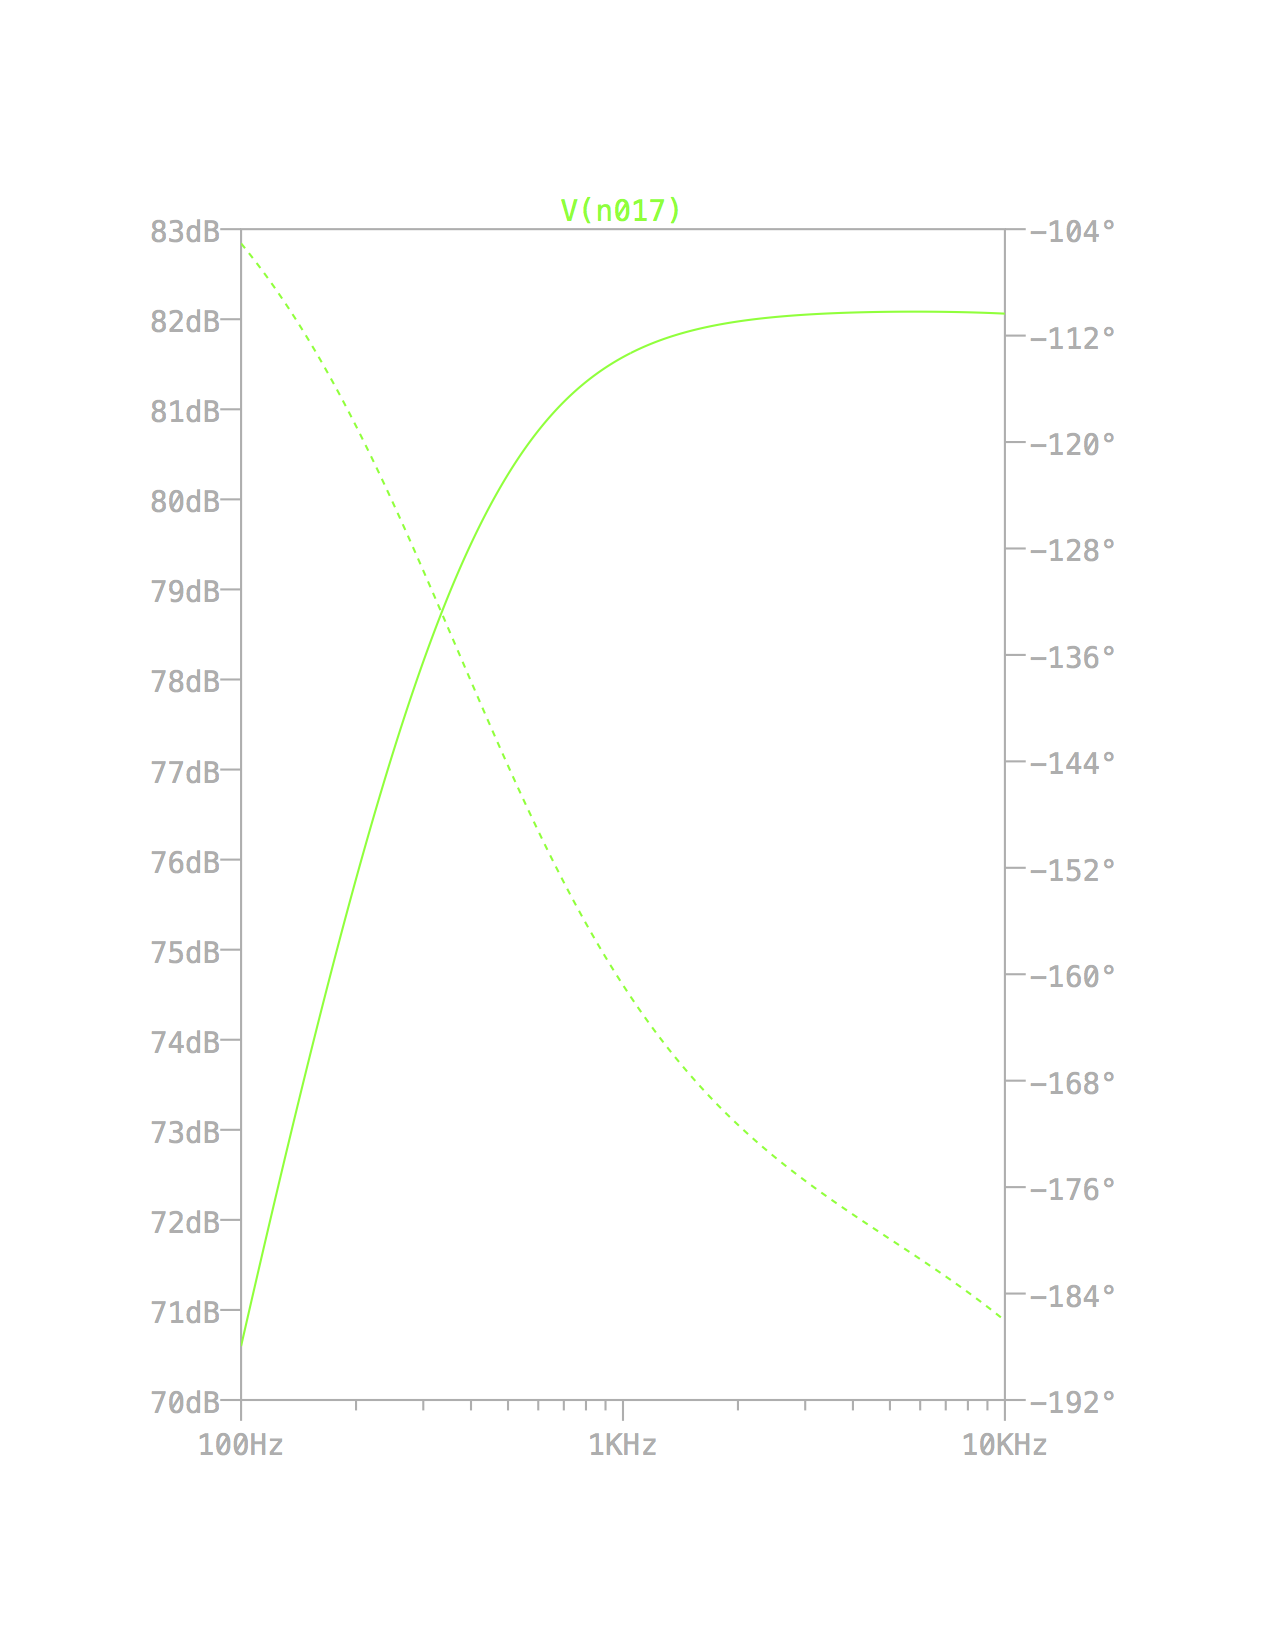
\includegraphics[width=7in]{MagPlot.png}
\caption{Magnitude (Solid Line) and Phase (Dotted Line) Plot from SPICE}
\end{center}
\end{figure}
\FloatBarrier

\begin{figure}
\begin{center}
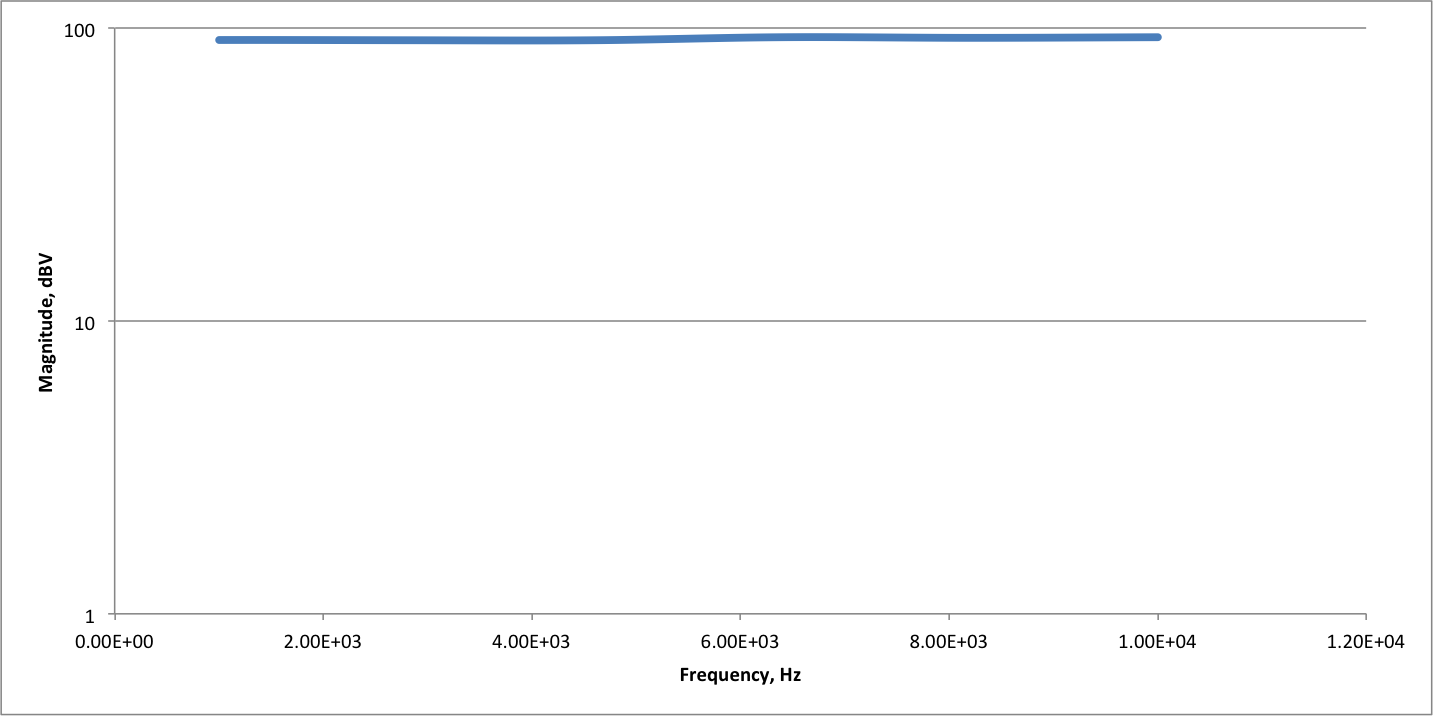
\includegraphics[width=7in]{measuredmag.png}
\caption{Measured Magnitude Plot}
\end{center}
\end{figure}

\begin{figure}[htbp]
\begin{center}
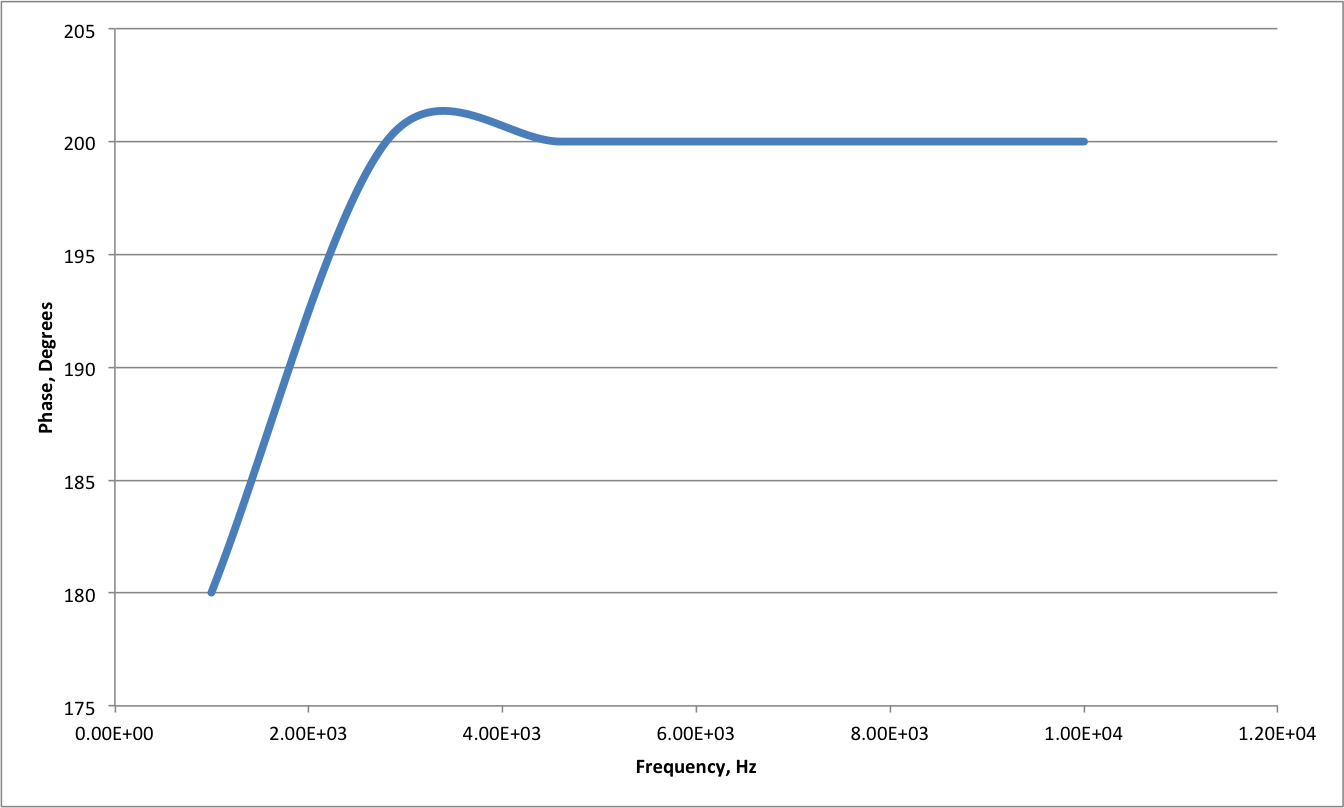
\includegraphics[width=7in]{measuredphase.png}
\caption{Measured Phase Plot}
\end{center}
\end{figure}
\FloatBarrier

\subsection*{Output Impedance}
Measured output impedance: $940 \Omega$
\subsection*{Bias Voltages/Currents}
\begin{tabular}{|r|l|l|}
\hline
Stage & $V_{GS}$ & Drain Current\\
\hline
Stage 1 &2.32V&6.2mA\\
Stage 2 &2.4V&6.2mA\\
Stage 3 &2.37V&5.14mA\\
Stage 4 &2.48V&4.55mA\\
Stage 5 &4.7V&41mA\\
Stage 6 &2.8V&35mA\\
\hline
\end{tabular}

\begin{tabular}{|r|l|l|}
\hline
Stage & $V_{G}$ & Drain Current\\
\hline
Stage 1 &2.9V&6.09mA\\
Stage 2 &2.4V&6.2mA\\
Stage 3 &2.37V&5.14mA\\
Stage 4 &2.48V&4.55mA\\
Stage 5 &4.7V&41mA\\
\hline
\end{tabular}


\subsection*{Power Consumption}

\end{document}
